\documentclass{article}

\usepackage{graphicx}
\usepackage{subcaption}
\usepackage{listings}
\usepackage{amsmath}
\usepackage{cleveref}

\begin{document}


\subsection*{Problem 1}

\begin{figure}[h!]
	\centering
	\begin{subfigure}{0.4\linewidth}
		\includegraphics[width=\linewidth]{images/pic1.jpg}
		\caption{Perspective projection: Parallell lines are not parallell in the image}
	\end{subfigure}
	\begin{subfigure}{0.4\linewidth}
		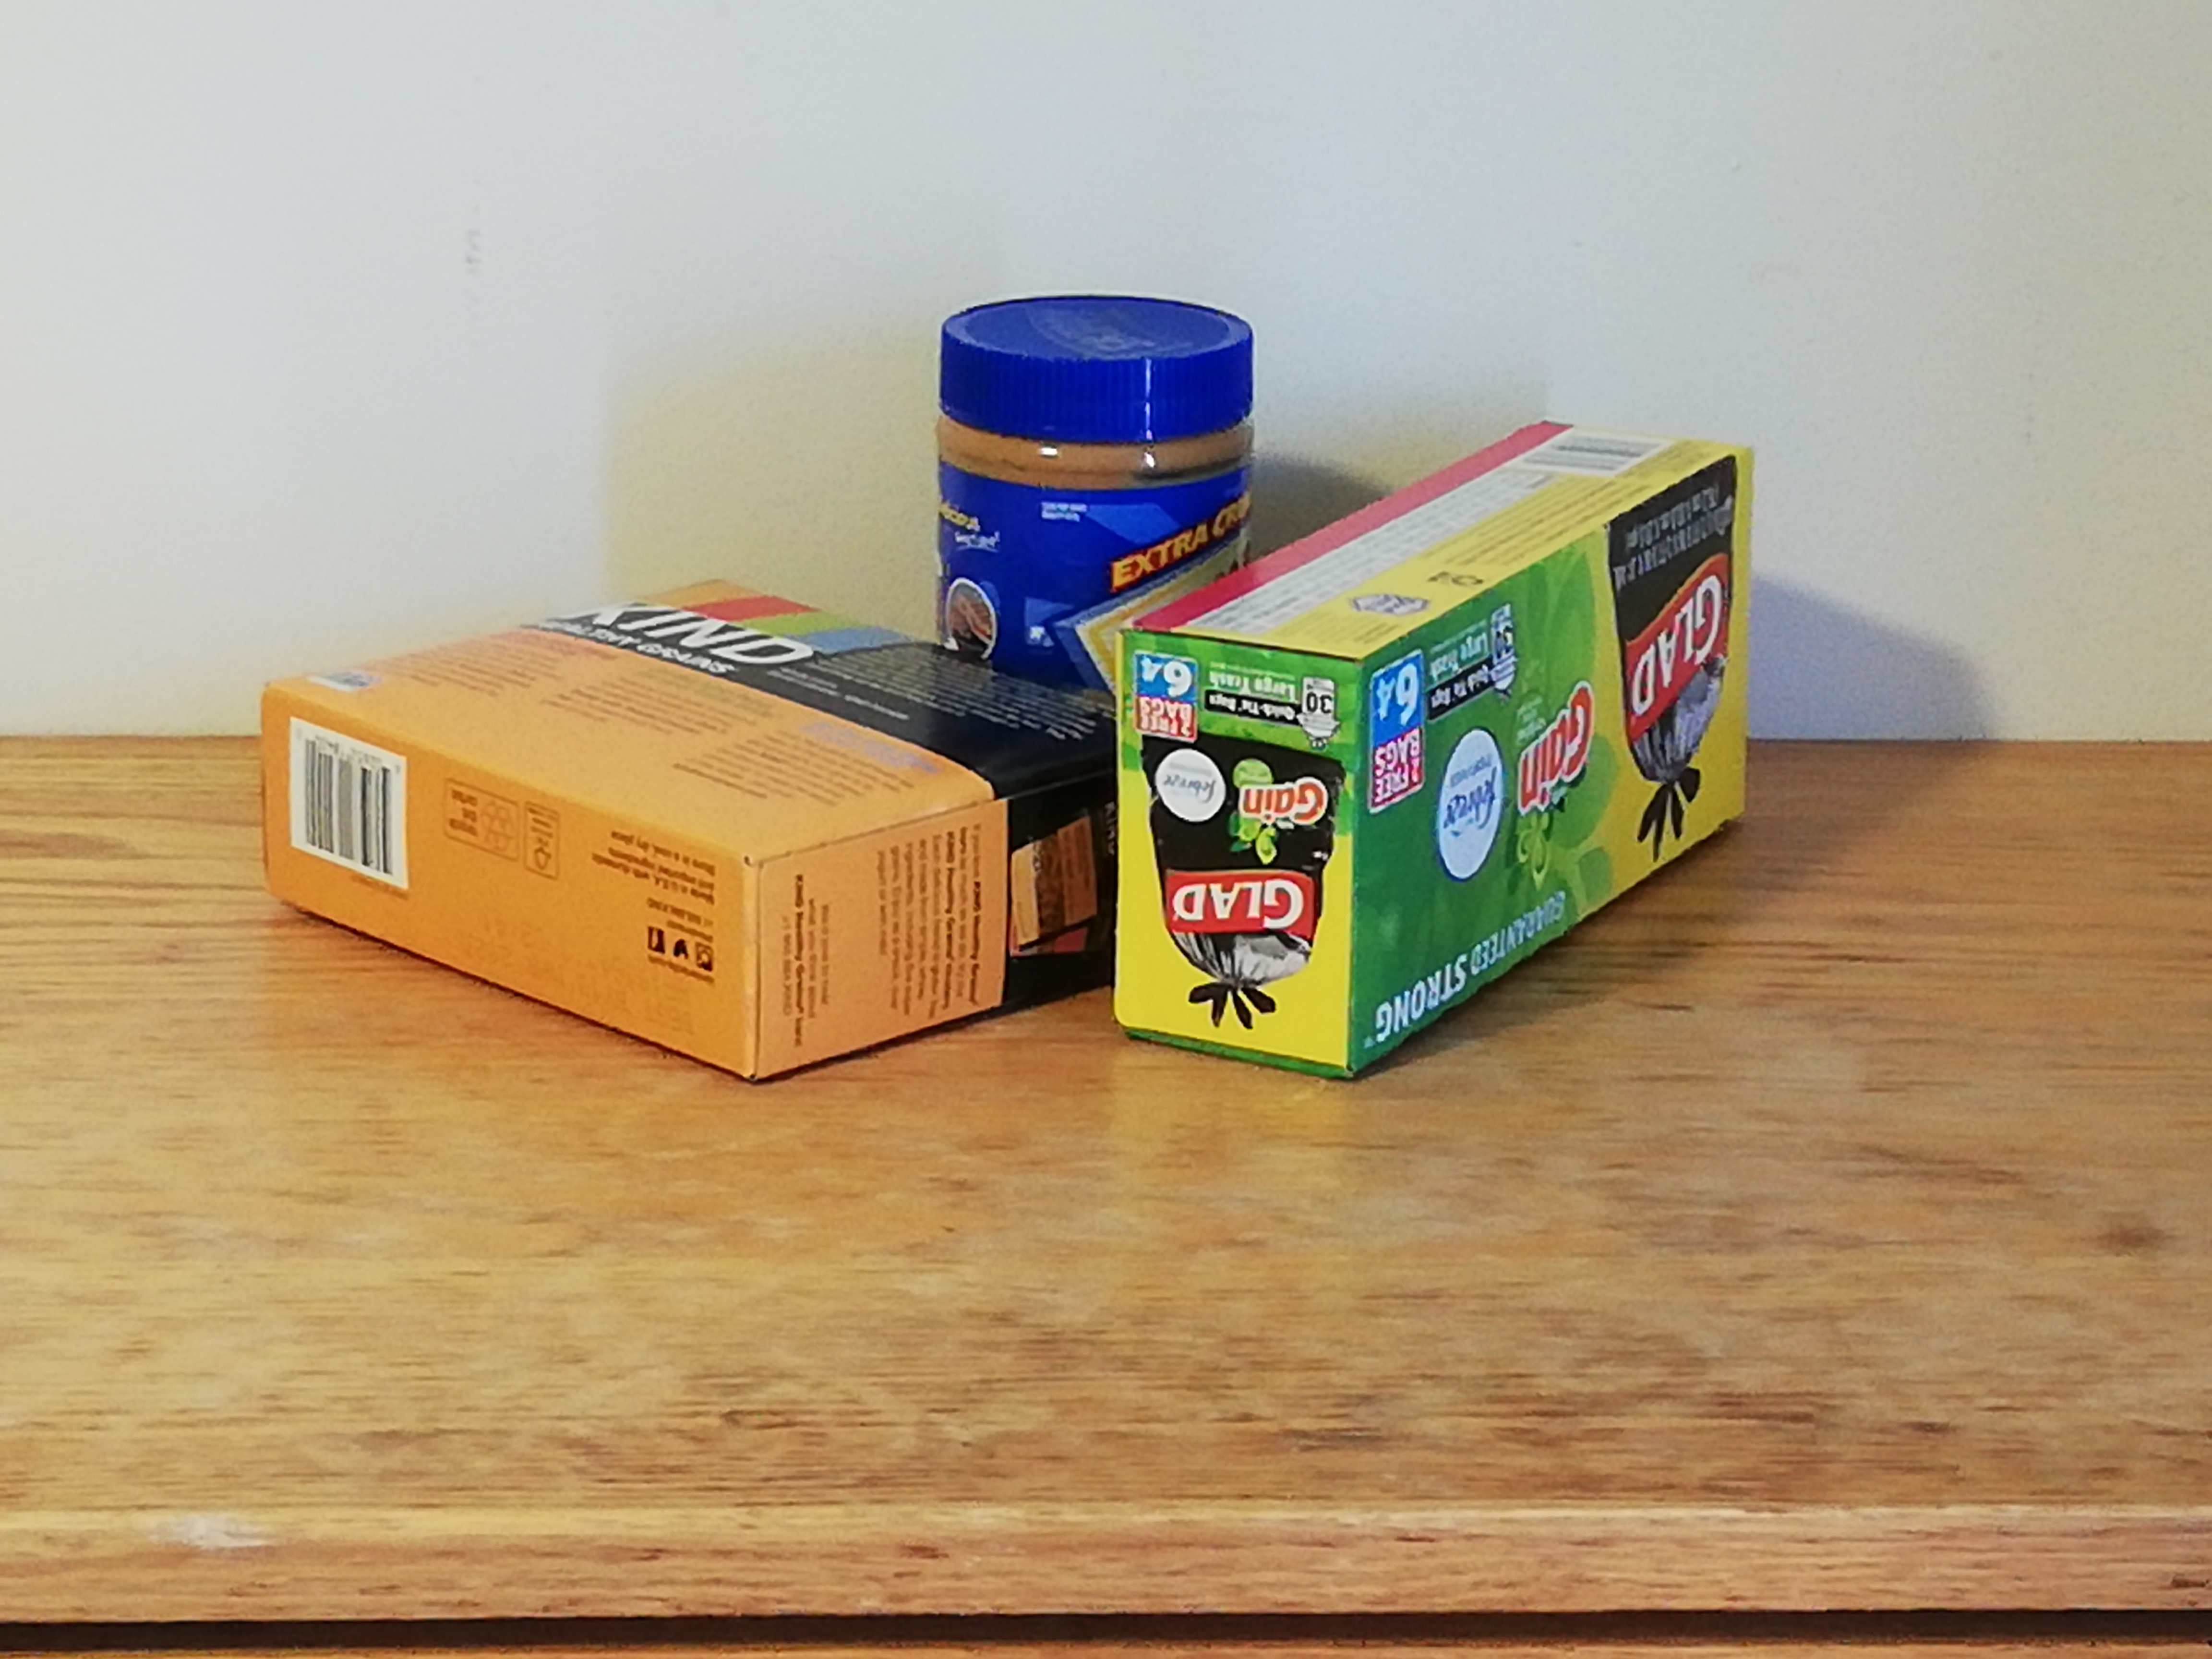
\includegraphics[width=\linewidth]{images/pic2.jpg}
		\caption{Orthographic projection: Parallell lines stay parallell in the image}
	\end{subfigure}
\end{figure}
The image to the left is taken normally, while the image to the right is taken from a distance with zoom. On the square boxes one can clearly see the difference. In the perspective projection the edges are converging to the vanishing points, while in the orthographic projection the edges are (approximately) parallell.


\subsection*{Problem 2}

Since a parallell projection simply translates the image from the world coordinate system to the virtual cameraplane, we can find the equations by rotating the world coordinate frame such that it is identically oriented as the camera system. In our case, this is a simple rotation around the X-axis by $-\theta$, with positive direction defined as normal for right-handed systems.

\begin{equation}
	\begin{bmatrix}
		x \\
		y \\
		z \\
	\end{bmatrix}
	=
	\begin{bmatrix}
		1 & 0 & 0\\
		0 & \cos(-\theta) & \sin(-\theta)\\
		0 & -\sin(-\theta) & \cos(-\theta)\\
	\end{bmatrix}
	\begin{bmatrix}
		X \\ Y \\ Z
	\end{bmatrix}
\end{equation}

This gives $x=X$ and $y=\cos(\theta)Y - \sin(\theta)Z$. When changing to square pixels, the coordinates will be scaled by some factor $\alpha$. And since the origin in the virtual cameraplane plane does not need to be aligned with the world origin, we must also add offsets $x_0$ and $y_0$ resulting in

\begin{equation}
\begin{split}
	x &= \alpha X + x_0 \\
	y &= \alpha(\cos(\theta)Y - \sin(\theta)Z) + y_0
\end{split}
\label{eq:x_y}
\end{equation}

\subsection*{Problem 3}

By our assumption, all vertical edges in the image is vertical in the world. Since $Z$ is constant along vertical edges we get

\begin{equation}
\begin{split}
	\frac{\partial Z}{\partial y} &= 0
\end{split}
\end{equation}
From \cref{eq:x_y} we can find the constraint on horizontal edges. Differentiating along the edge given by $t$ as in the notes gives
\begin{equation}
\begin{split}
	n_x &= -\alpha \sin(\theta) \frac{\partial Z}{\partial t}\\
	\frac{\partial Z}{\partial t} &= \frac{-n_x}{\alpha\sin(\theta)}
\end{split}
\end{equation}

As for $Y$, the assumption of planar surfaces means the second derivatives must be zero

\begin{equation}
\begin{split}
	\frac{\partial^2 Z}{\partial x^2} &= 0 \\
	\frac{\partial^2 Z}{\partial y^2} &= 0 \\
	\frac{\partial^2 Z}{\partial x \partial y} &= 0
\end{split}
\end{equation}


\subsection*{Problem 4}
\begin{lstlisting}[language=Python]
# Line 51
Aij[:,:,c] = 
	- ny*np.array([[-1, 0, 1], [-2, 0, 2], [-1, 0, 1]])/8
	+ nx*np.array([[-1, -2, -1], [0, 0, 0], [1, 2, 1]])/8;
	
# Line 65
Aij[:,:,c] = 
	0.1*np.array([[0, -1, 0], [0, 2, 0], [0, -1, 0]]);
\end{lstlisting}

The first kernel corresponds to $-n_y\partial Y / \partial x + n_x\partial Y / \partial y$, while the second corresponds to $\partial^2 Y / \partial y^2$.\\

\subsection*{Problem 5}

\begin{figure}[h!]
	\centering
	\begin{subfigure}{0.4\linewidth}
		\includegraphics[width=\linewidth]{images/img2_rotated.png}
		\caption{Image 2 as seen from a new perspective}
		\label{fig:p51}
	\end{subfigure}
	\begin{subfigure}{0.4\linewidth}
		\includegraphics[width=\linewidth]{images/steps_rotated.png}
		\caption{Image of the steps, as seen from a new perspective}
		\label{fig:p52}
	\end{subfigure}
	\caption{Rotated images rendered back to 3D}
	\label{fig:p5}
\end{figure}

Two of the rotated images can be seen in \cref{fig:p5}.


\subsection*{Problem 6}

\begin{figure}[ht!]
	\centering
	\begin{subfigure}{0.6\linewidth}
		\includegraphics[width=\linewidth]{images/img4_flat.png}
		\caption{Image 4 as seen from a new perspective}
			\label{fig:p6_figa}
	\end{subfigure}
	\begin{subfigure}{0.6\linewidth}
		\includegraphics[width=\linewidth]{images/img4_flat_edges.png}
		\caption{The detected edges in image 4}
			\label{fig:p6_figb}
	\end{subfigure}
	\begin{subfigure}{0.6\linewidth}
		\includegraphics[width=\linewidth]{images/img4_flat_shaded.png}
		\caption{Coordinate gradients for image 4}
			\label{fig:p6_figc}
	\end{subfigure}
	\caption{Recovered 3D information from image 4}
\end{figure}

In \cref{fig:p6_figa} you can see how the recovery of image 4 fails. The orange and blue boxes appears to be surfaces in 3D space, and the green cube apprears flat in the $XZ$-plane. The distortion of the blue and orange boxes comes from the models inability to infer the unseen parts of objects, as this would require semantic knowledge about the world and the object in question. From \cref{fig:p6_figb} it seems the model is not detecting all the vertical edges on the green box properly. This causes the top of the green box to be interpreted as ground level as seen in the $Y$ gradient in \cref{fig:p6_figc}


\subsection*{Problem 7}

One of the many assumptions we made for the simple vision system was that all surfaces is planar. If we try to use this vision model on something like a cylinder we get incorrect, but hilarious results as the one seen in \cref{fig:dist_cylinder}. The model tried to explain such a shape by modeling it as a planar surface going up and towards the camera. 

We could approximate the curvature of an edge by considering the normal vectors in a small neighbourhood around each point along the edge. Then perhaps the curvature at a surface point could be estimated by some interpolation of surrounding edges. 

\begin{figure}[h!]
	\centering
	\begin{subfigure}{0.4\linewidth}
		\includegraphics[width=\linewidth]{images/cylinder_levels.png}
		\caption{Coordinate gradients for the cylinder}
	\end{subfigure}
	\begin{subfigure}{0.4\linewidth}
		\includegraphics[width=\linewidth]{images/flat_cylindre.png}
		\caption{Distorted cylinder rendered back to 3D}
		\label{fig:dist_cylinder}
	\end{subfigure}
	\caption{Reconstructed sylinder coordinates}
\end{figure}

\end{document}
